% !TEX TS-program = pdflatexmk
\documentclass{article}
\usepackage[latin1]{inputenc} 

\newenvironment{Ncenter}{%
  \setlength\topsep{-10pt}
  \setlength\parskip{-100pt}
  \begin{center}
}{%
  \end{center}
}


\newcommand{\kmo}{k_{\mathrm{OT \to O+T}}}
\newcommand{\kOpT}{k_{\mathrm{O+T \to OT}}}
\newcommand{\kmt}{k_{\mathrm{OTE \to OT+E}}}
\newcommand{\kt}{k_{\mathrm{OT+E \to OTE}}}
\newcommand{\kE}{k_{\mathrm{OTE \to OCE}}}
\newcommand{\kD}{k_{\mathrm{OC \to O+C}}}
\newcommand{\vp}{v_{\mathrm{prod}}}
\newcommand{\vd}{k_{\mathrm{T \to \emptyset}}}
\newcommand{\Trel}{T_{\rm{rel}}}
\newcommand{\EC}{EC_{\rm{50}}}
\newcommand{\KdOT}{K_{\mathrm{dOT}}}
\newcommand{\Trelmin}{T_{\rm{rel,min}}}

\usepackage[labelsep=none]{caption}
\renewcommand{\thefigure}{}

\title{R-code for producing Figure 2 from Pedersen et al. (2013)}
\author{Lykke Pedersen, \and Peter H Hagedorn, \and Marie Lindholm, \and Morten Lindow}
\date{}

\usepackage{Sweave}
\begin{document}
\Sconcordance{concordance:Vignette2.tex:Vignette2.Rnw:%
1 33 1 1 0 6 1 1 2 1 0 1 2 4 0 1 2 3 1 1 3 2 0 1 2 1 0 1 1 3 0 2 2 4 0 %
2 2 1 0 1 2 1 0 1 2 1 1 1 3 1 0 1 6 5 0 1 1 1 2 1 0 3 1 1 3 2 0 1 3 2 0 %
1 3 2 0 1 3 2 0 1 3 5 0 1 2 8 1 1 2 1 0 1 3 2 0 2 1 1 2 1 0 2 1 3 0 1 2 %
9 1 1 2 1 0 1 1 3 0 2 2 1 0 2 1 3 0 2 2 1 0 1 2 1 0 2 1 1 2 1 0 1 1 3 0 %
1 2 8 1 1 2 1 0 3 1 1 3 1 0 1 1 2 2 1 3 2 0 1 2 6 1 1 2 1 0 2 1 3 0 1 2 %
7 1 1 3 2 0 1 1 1 2 1 1 1 2 1 0 1 2 1 0 1 2 1 3 2 0 5 1 1 2 1 0 2 1 3 0 %
1 2 7 1 1 3 2 0 1 1 3 2 1 0 1 1 1 2 7 1 1 2 1 0 2 1 3 0 1 2 77 1}



\maketitle
This vignette includes the commands to reproduce Fig. 2 from ``A kinetic model explains why shorter and less
affine enzyme-recruiting oligonucleotides can be
more potent". The R-functions from the ASOmodels package are used.
\begin{Schunk}
\begin{Sinput}
> require(devtools)
> #install_github('ASOmodel',username='lykkep',build=FALSE)
> require(ASOmodels)
\end{Sinput}
\end{Schunk}

%%%%%%%%%%%%%%%%%%%%%%%%%%%%%%%%%%%%%%%%%%%%%%%%%%%%%%%%%%%%%%%%%%%%%%%%%%
\section*{Kinetic model figures}

%%%%%%%%%%%%%%%%%%%%%%%%%%%%%%%%%%%%%%%%%%%%%%%%%%%%%%%%%%%%%%%%%%%%%%%%%%
\subsection*{Figure 2a: Time-resolved simulation of the model (unsaturated)}
Parameters for the model, the initial concentrations and the time-steps for which the simulation is performed:
\begin{Schunk}
\begin{Sinput}
> parms <- c(Et = 1,KdOT = 0.3,kOpT = 0.2,KdOTE = 70,kOTpE = 5,  
+            vprod = 0.2,kdegrad = 0.04,alpha=0.1,kcleav = 8)
> init <- c(T=parms['vprod']/parms['kdegrad'], OT=0, OTE=0, 
+           E=parms['Et'], O=0.1, OCE=0, OC=0)
\end{Sinput}
\end{Schunk}
Using \texttt{vode()} the model is simulated in time. The function \texttt{diffASO()} is part of the ASOmodels package. 
\begin{Schunk}
\begin{Sinput}
> solASO <- vode(init,0:100,diffASO,parms)
\end{Sinput}
\end{Schunk}
The timetraces for the concentrations of $[O]$, $[T]$, $[OT]$, $[OTE]$, and $[E]$ are plotted:
\begin{Schunk}
\begin{Sinput}
> colVAR <- c("black","darkgreen","darkred","orange","green")  
> SSvalue <- signif(last(solASO),3) 
> SSvalue[c(3:4,6)] <- SSvalue[c(3:4,6)]*1E3
> xtime <- 59; ySS <- c(0.08,0.88,0.83,0.18,0.13)
> uSS <- c('nM','pM','pM','nM','pM')
> labSS=c('T','OT','OTE','E','O')
> par(mar=c(3.2,3.4,0.1,0.1),bty='n',mgp=c(2,0.7,0),
+     las=1,cex.lab=1.25)
> plot(0,0,ylim=c(0,1),xlim=c(0,xtime+30),type='n',xaxt='n',
+      yaxt='n',ylab='relative concentrations',xlab='minutes')
> axis(2,at=c(0,1),label=c('min','max'),las=1)
> axis(1,at=c(seq(0,xtime,by=10),xtime+20),
+      label=c(seq(0,xtime,by=10),''))
> axis(1,at=xtime+20,label='steady-\nstate',mgp=c(0,1.6,0))
> for(i in 2:6){ 
+   par(new=TRUE)
+   plot(solASO[1:(xtime+1),1], solASO[1:(xtime+1),i], xaxt='n',
+        yaxt='n',ylim=range(solASO[,i]),col=colVAR[i-1], 
+        type='l',ylab=NA,xlab=NA,xlim=c(0,xtime+30)) 
+   lines(xtime+5:37,rep(solASO[101,i],33),col=colVAR[(i-1)]) 
+   y <- diff(par('usr')[3:4])*ySS[i-1]+par('usr')[3]
+   text(xtime+5,y,col=colVAR[i-1],adj=0,cex=0.8,
+        substitute(b==e*l,list(e=SSvalue[i],l=uSS[i-1],b=labSS[i-1]) ))
+ }
\end{Sinput}
\end{Schunk}
\begin{figure}[!h]
\begin{Ncenter}
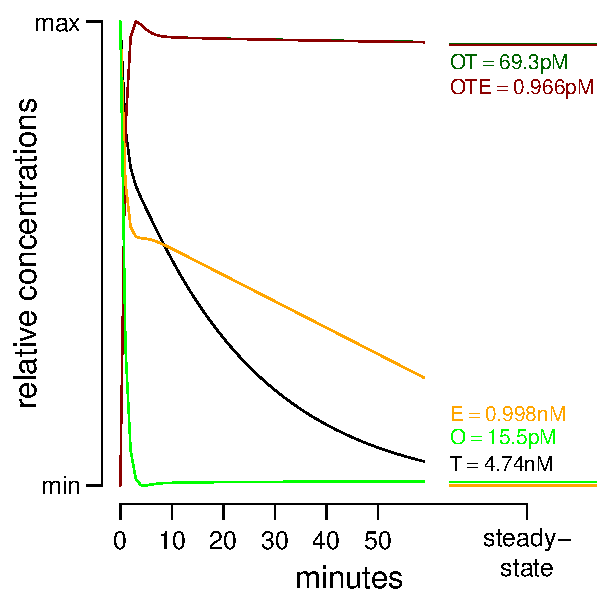
\includegraphics[width=0.5\textwidth]{Vignette2-Figa}
\end{Ncenter}
\caption{2a: Time resolved simulation of the relative concentrations of key species.}
\end{figure}

%%%%%%%%%%%%%%%%%%%%%%%%%%%%%%%%%%%%%%%%%%%%%%%%%%%%%%%%%%%%%%%%%%%%%%%%%%
\subsection*{Figure 2b: Time-resolved simulation of the model (saturated)}
The initial oligonucleotide concentration is increased to 100nM.
\begin{Schunk}
\begin{Sinput}
> init <- c(T=parms['vprod']/parms['kdegrad'], OT=0, OTE=0, 
+           E=parms['Et'], O=100, OCE=0, OC=0)
> solASO <- vode(init,0:100,diffASO,parms)
\end{Sinput}
\end{Schunk}
The timetraces for the concentrations of $[O]$, $[T]$, $[OT]$, $[OTE]$, and $[E]$ are plotted:
\begin{Schunk}
\begin{Sinput}
> SSvalue <- signif(last(solASO),3)
> SSvalue[c(2,4)] <- SSvalue[c(2,4)]*1E3
> xtime <- 55; ySS <- c(0.06,0.3,0.34,0.26,0.67)
> uSS <- c('pM','nM','pM',rep('nM',2)) 
> labSS=c('T','OT','OTE','E','O')
> par(mar=c(3.2,3.4,0.1,0.1),bty='n',mgp=c(2,0.7,0),
+     las=1,cex.lab=1.25)
> plot(0,0,ylim=c(0,1),xlim=c(0,xtime+25),type='n',xaxt='n',
+      yaxt='n',ylab='relative concentrations',xlab='minutes')
> axis(2,at=c(0,1),label=c('min','max'),las=1)
> axis(1,at=c(seq(0,xtime,by=10),xtime+15),
+      label=c(seq(0,xtime,by=10),''))
> axis(1,at=xtime+15,label='steady-\nstate',mgp=c(0,1.6,0))
> for(i in 2:6){ 
+   par(new=TRUE)
+   plot(solASO[1:(xtime+1),1], solASO[1:(xtime+1),i], xaxt='n',
+        yaxt='n',ylim=range(solASO[,i]),col=colVAR[i-1], 
+        type='l',ylab=NA,xlab=NA,xlim=c(0,xtime+25)) 
+   lines(xtime+5:25,rep(solASO[101,i],21),col=colVAR[(i-1)]) 
+   y <- diff(par('usr')[3:4])*ySS[i-1]+par('usr')[3]
+   text(xtime+5,y,col=colVAR[i-1],adj=0,cex=0.8,
+        substitute(b==e*l,list(e=SSvalue[i],l=uSS[i-1],b=labSS[i-1])))
+ }
\end{Sinput}
\end{Schunk}
\begin{figure}[!h]
\begin{Ncenter}
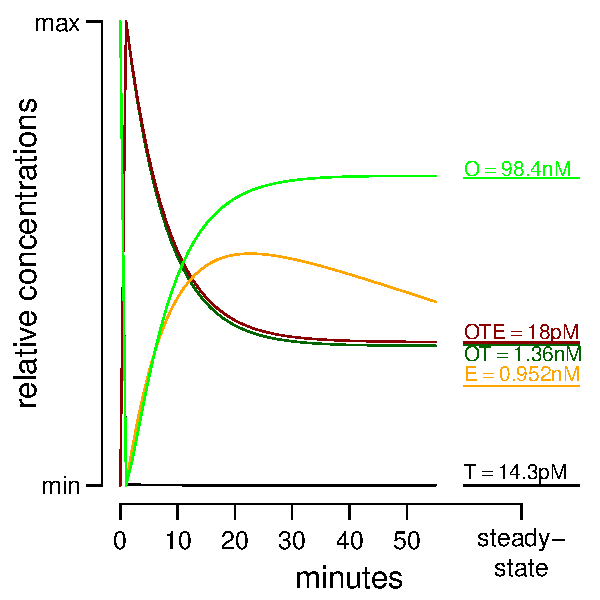
\includegraphics[width=0.5\textwidth]{Vignette2-Figb}
\end{Ncenter}
\caption{2b: Time resolved simulation of the relative concentrations of key species.}
\end{figure}
\newpage

%%%%%%%%%%%%%%%%%%%%%%%%%%%%%%%%%%%%%%%%%%%%%%%%%%%%%%%%%%%%%%%%%%%%%%%%%%
\subsection*{Figure 2c: Simulated dose-response curve}
Given a set of parameters the R-function \texttt{Trel()} from the ASOmodels package calculates the relative target concentration as a function of the total concentration of oligonucleotide added to the system.
\begin{Schunk}
\begin{Sinput}
> par(mar=c(3.2,3.4,0.1,0.1),bty='n',mgp=c(2,0.7,0),
+     las=1,cex.lab=1.25)
> curve(Trel,1E-3,5E2,log='x', lwd=2,ylim=c(0,1),
+       ylab=expression(T[rel]),xaxt='n',
+       xlab='Total oligonucleotide conc (nM)')
> abline(h=Trel(1E9),lty=2) #Trel,min
> abline(v=EC50(parms['KdOT']),lty=2) #EC50
> axis(1,at=10^c(-3,-1,1,3),
+      labels=pretty10expLP(10^c(-3,-1,1,3),drop.1=T))
> axis(1,at=EC50(parms['KdOT']),label=expression(EC[50]))
> axis(2,at=Trel(1E6),label=expression(T[rel*','*min]),las=1)
\end{Sinput}
\end{Schunk}
\begin{figure}[!h]
\begin{Ncenter}
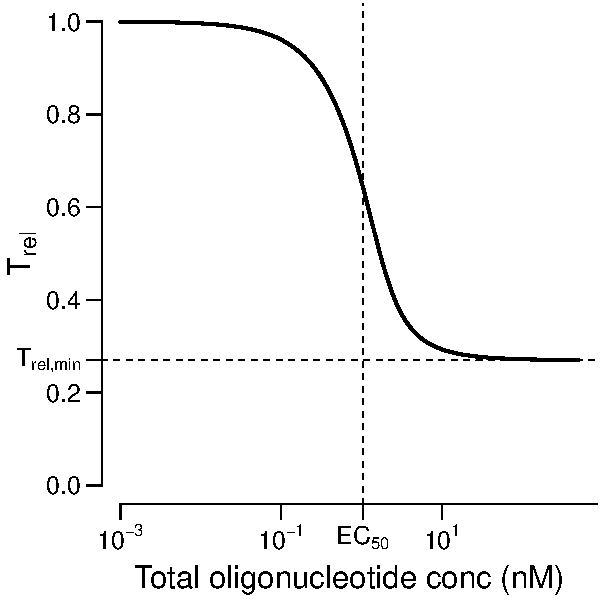
\includegraphics[width=0.5\textwidth]{Vignette2-Figc}
\end{Ncenter}
\caption{2c: The relative total target concentration ($\Trel$) is defined as the steady state level of total target in the presence of oligonucleotide divided by the target concentration in the absence of oligonucleotide. Dashed lines indicate 1-efficacy (horizontal) and $\EC$ (vertical).}
\end{figure}

%%%%%%%%%%%%%%%%%%%%%%%%%%%%%%%%%%%%%%%%%%%%%%%%%%%%%%%%%%%%%%%%%%%%%%%%%%
\subsection*{Figure 2d: An optimal affinity}
For a range of affinities \texttt{D1\_seq} the $\EC$-values are calculated by use of the R-function \texttt{EC50()} from the ASOmodels package:
\begin{Schunk}
\begin{Sinput}
> D1_seq <- 10^seq(-3,3,by=0.25)
> ECfit <- sapply(D1_seq,EC50)
\end{Sinput}
\end{Schunk}
When there is no coupling between the off-rates $\kmo$ and $\kD$ then the value of $\kD$ is set in the param vector as the entry \texttt{'kC'}:
\begin{Schunk}
\begin{Sinput}
> parmsNO <- c(parms,kC=parms['kOpT']*parms['KdOT']/parms['alpha'])
> names(parmsNO)[length(parmsNO)] <- 'kC'
> ECfitNO <- sapply(D1_seq,EC50NO) #EC50 without coupling
\end{Sinput}
\end{Schunk}
For the range of affinities the corresponding $\EC$-values are plotted:
\begin{Schunk}
\begin{Sinput}
> par(mar=c(3.2,3.4,0.1,0.1),bty='n',mgp=c(2,0.7,0),
+     las=1,cex.lab=1.25)
> plot(D1_seq,ECfit,log='xy',yaxt='n',type='l',xaxt='n',
+      xlab=expression(K[dOT]~'(nM)'),
+      ylab=expression(EC[50]~'(nM)'))
> lines(D1_seq,ECfitNO,lty=2)
> axis(2,at=c(2,20,200),labels=c(2,20,200),las=2)
> axis(1,at=10^pretty(log10(D1_seq)),
+      labels=pretty10expLP(10^pretty(log10(D1_seq)),drop.1=T),)
> legend('topleft',c('Coupling','No coupling'),lty=c(1,2),bty='n')
\end{Sinput}
\end{Schunk}
\begin{figure}[!h]
\begin{Ncenter}
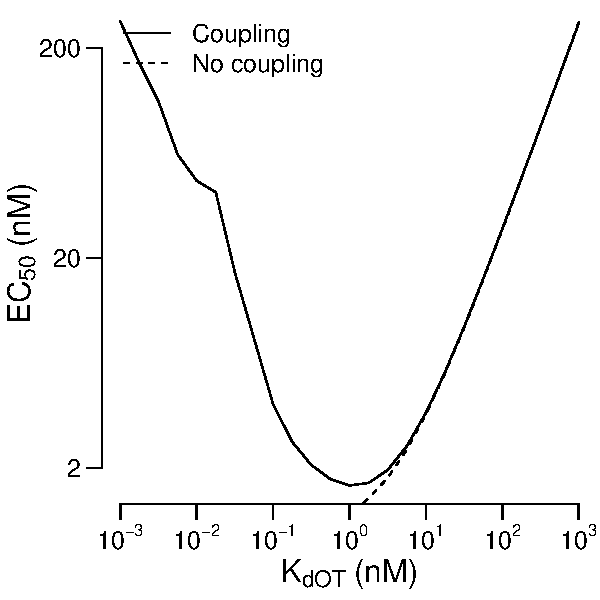
\includegraphics[width=0.5\textwidth]{Vignette2-Figd}
\end{Ncenter}
\caption{2d: $\EC$ as a function of the dissociation constant for the OT complex. A low $\KdOT$ corresponds to a high affinity binding. Dashed line: no coupling of off-rates. Solid line: coupling of off-rates.}
\end{figure}

%%%%%%%%%%%%%%%%%%%%%%%%%%%%%%%%%%%%%%%%%%%%%%%%%%%%%%%%%%%%%%%%%%%%%%%%%%
\section*{Experimental data figures}

%%%%%%%%%%%%%%%%%%%%%%%%%%%%%%%%%%%%%%%%%%%%%%%%%%%%%%%%%%%%%%%%%%%%%%%%%%
\subsection*{Figure 2e: Frieden et al. (2003)}
\begin{Schunk}
\begin{Sinput}
> data(gapmers)
> dat <- data.frame(gapmers)
> colL <- c('red','orange','darkgreen','','darkblue','',
+           'purple','','black')
> OLength <- sort(unique(dat$Oligo.length))
> #### We plot the data from Frieden et al, 2003
> dat.F <- dat[dat$Study=="Frieden 2003",]
> Flength <- dat.F$Oligo.length
> par(mar=c(3.2,3.4,0.1,0.1),bty='n',mgp=c(2,0.7,0),
+     las=1,cex.lab=1.25)
> fitpar <- function(x,y){
+   Fit <- lm(y ~ x + I(x^2))
+   coef <- coefficients(Fit)
+   f <- summary(Fit)$fstatistic
+   p <- signif(pf(f[1],f[2],f[3],lower.tail=F),2)
+   xmin <- round(-coef[2]/(2*coef[3]))
+   tmp <- as.expression(substitute(Optimal~T[m]%~~%x*degree*C,list(x=xmin)))
+   return(list(coef=coef,p=p,legend=tmp))
+ }
> Fx <- dat.F$Predicted.Tm; Fy <- dat.F$Dose.2nm
> FitF <- fitpar(Fx,Fy)
> Parfun <- function(x){FitF$coef[1]+FitF$coef[2]*x+FitF$coef[3]*x^2}
> curve(Parfun(x),min(Fx),max(Fx), lwd=1,col='grey',ylim=c(0,110),
+      ylab='activity (% of control)',
+      xlab=expression('predicted'~T[m]~'('*degree*'C)'))
> legend(diff(par('usr')[1:2])/2+par('usr')[1],100,
+        c('Luciferase',paste('p =',FitF$p),FitF$legend), 
+        bty='n',cex=1.1,yjust=0.4,xjust=0.5  )
> points(Fx,Fy,pch=19,cex=2,col=colL[Flength-11])
\end{Sinput}
\end{Schunk}
\begin{figure}[!h]
\begin{Ncenter}
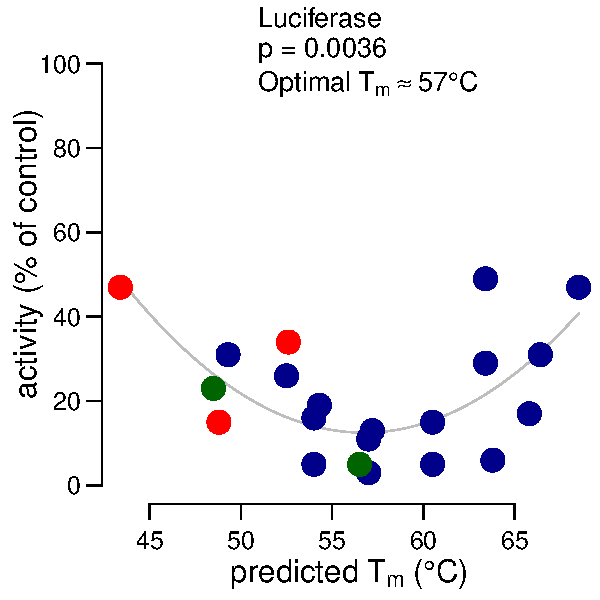
\includegraphics[width=0.5\textwidth]{Vignette2-Fige}
\end{Ncenter}
\caption{2e:  21 oligonucleotides targeted against the luciferase firefly gene.}
\end{figure}

%%%%%%%%%%%%%%%%%%%%%%%%%%%%%%%%%%%%%%%%%%%%%%%%%%%%%%%%%%%%%%%%%%%%%%%%%%
\section*{Figure 2f: Stanton et al. (2012)}
\begin{Schunk}
\begin{Sinput}
> #### We plot the data from Stanton et al 2012
> dat.S <- dat[dat[,1]=="Stanton 2012",]
> Slength <- dat.S$Oligo.length
> par(mar=c(3.2,3.4,0.1,0.1),bty='n',mgp=c(2,0.7,0),
+     las=1,cex.lab=1.25)
> Sx <- dat.S$Predicted.Tm; Sy <- dat.S$Dose.3nm
> FitS <- fitpar(Sx,Sy)
> Parfun <- function(x){FitS$coef[1]+FitS$coef[2]*x+FitS$coef[3]*x^2}
> curve(Parfun(x),min(Sx),max(Sx), lwd=1,col='grey',,ylim=c(0,110),
+      ylab='mRNA (% of control)', 
+      xlab=expression('predicted'~T[m]~'('*degree*'C)'))
> points(Sx,Sy, pch=19,col=colL[Slength-11],cex=2)
> legend('bottomright',as.character(sort(unique(OLength))),
+        pch=19,col=colL[sort(unique(OLength))-11],bg='white',
+        horiz=T,bty='n',cex=1.1)
> legend(diff(par('usr')[1:2])/2+par('usr')[1],100,
+        c('GR',paste('p =',FitS$p),FitS$legend), 
+        bty='n',cex=1.1,yjust=0.4,xjust=0.5  )
\end{Sinput}
\end{Schunk}
\begin{figure}[!h]
\begin{Ncenter}
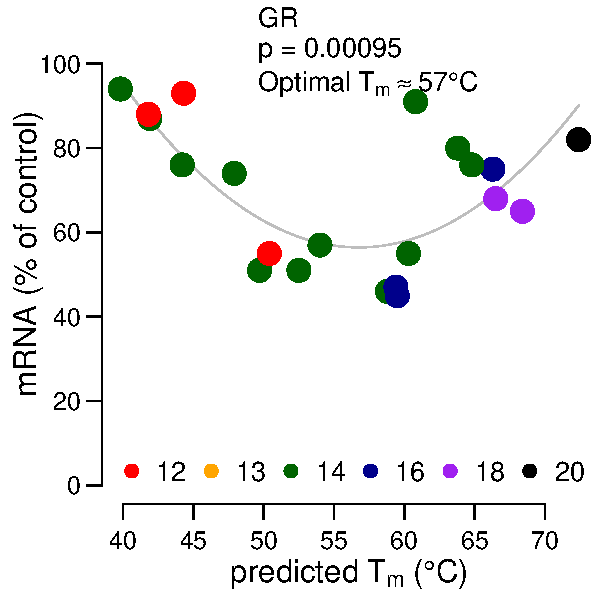
\includegraphics[width=0.5\textwidth]{Vignette2-Figf}
\end{Ncenter}
\caption{2f: 21 oligonucleotides targeted against the glucocorticoid receptor.}
\end{figure}

%%%%%%%%%%%%%%%%%%%%%%%%%%%%%%%%%%%%%%%%%%%%%%%%%%%%%%%%%%%%%%%%%%%%%%%%%%
\section*{Figure 2g: Pedersen et al. (2013) (this work)}
\begin{Schunk}
\begin{Sinput}
> ### We plot the data from Pedersen et al, 2013
> dat.P <- dat[dat$Study=="Pedersen 2013",]
> Plength <- dat.P$Oligo.length
> par(mar=c(3.2,3.4,0.1,0.1),bty='n',mgp=c(2,0.7,0),
+     las=1,cex.lab=1.25)
> Px <- dat.P$Predicted.Tm; Py <- dat.P$Dose.1nm
> FitP <- fitpar(Px,Py)
> Parfun <- function(x){FitP$coef[1]+FitP$coef[2]*x+FitP$coef[3]*x^2}
> curve(Parfun(x),min(Px),max(Px), lwd=1,col='grey',
+       xlab=expression('predicted'~T[m]~'('*degree*'C)'),
+      ylim=c(0,110),ylab='mRNA (% of control)' )
> points(Px,Py,pch=19,cex=2,col=colL[Plength-11],)
> legend(diff(par('usr')[1:2])/2+par('usr')[1],100,
+        c(expression('APOB ('*O[t]=='1nM)'),paste('p =',FitP$p),FitP$legend), 
+        bty='n',cex=1.1,yjust=0.4,xjust=0.5 )
\end{Sinput}
\end{Schunk}
\begin{figure}[!h]
\begin{Ncenter}
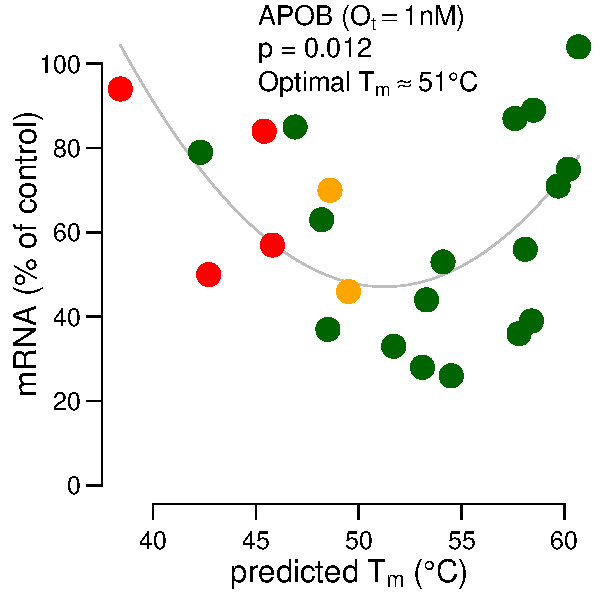
\includegraphics[width=0.5\textwidth]{Vignette2-Figg}
\end{Ncenter}
\caption{2g: 23 oligonucleotides targeted against apolipoprotein B.}
\end{figure}

%%%%%%%%%%%%%%%%%%%%%%%%%%%%%%%%%%%%%%%%%%%%%%%%%%%%%%%%%%%%%%%%%%%%%%%%%%
\section*{Figure 2h: Pedersen et al. (2013) (this work)}
\begin{Schunk}
\begin{Sinput}
> ### We plot the data from Pedersen et al, 2013
> dat.P <- dat[dat$Study=="Pedersen 2013",]
> Plength <- dat.P$Oligo.length
> par(mar=c(3.2,3.4,0.1,0.1),bty='n',mgp=c(2,0.7,0),
+     las=1,cex.lab=1.25)
> Px <- dat.P$Predicted.Tm; Py <- dat.P$Dose.25nm
> FitP <- fitpar(Px,Py)
> Parfun <- function(x){FitP$coef[1]+FitP$coef[2]*x+FitP$coef[3]*x^2}
> curve(Parfun(x),min(Px),max(Px), lwd=1,col='grey',
+       xlab=expression('predicted'~T[m]~'('*degree*'C)'),
+      ylim=c(0,110),ylab='mRNA (% of control)' )
> points(Px,Py,pch=19,cex=2,col=colL[Plength-11],)
> legend(diff(par('usr')[1:2])/2+par('usr')[1],100,
+        c(expression('APOB ('*O[t]=='25nM)'),paste('p =',FitP$p),FitP$legend), 
+        bty='n',cex=1.1,yjust=0.4,xjust=0.5 )
\end{Sinput}
\end{Schunk}
\begin{figure}[!h]
\begin{Ncenter}
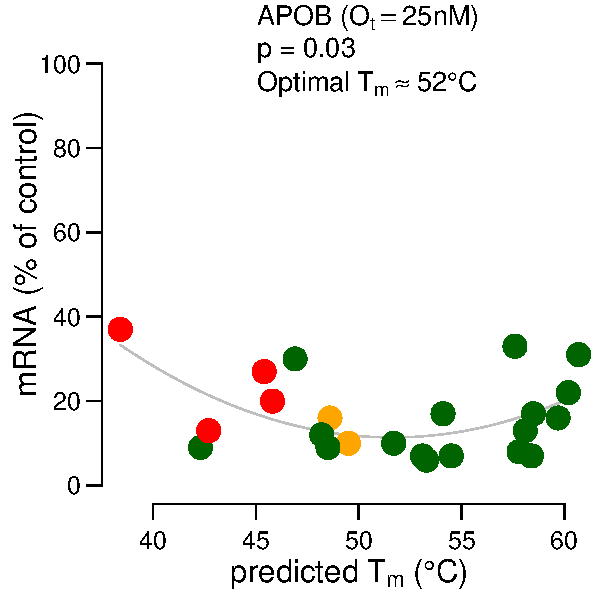
\includegraphics[width=0.5\textwidth]{Vignette2-Figh}
\end{Ncenter}
\caption{2h: 23 oligonucleotides targeted against apolipoprotein B.}
\end{figure}


% %%%%%%%%%%%%%%%%%%%%%%%%%%%%%%%%%%%%%%%%%%%%%%%%%%%%%%%%%%%%%%%%%%%%%%%%%%%%%
% % \section{Figure 4}
% % Supplementary Figure~\ref{fig::Opt} shows $\EC$ as a function of $\KdOT$ for various parameter values. It can be seen that the optimal affinity, quantified by $\KdOT$, changes as parameters are changed. A lower value of $\KdOT$ correponds to a better affinity for the oligonucleotide.
% % % % % %
% % % <<S2,echo=FALSE,fig=TRUE,include=FALSE,width=7,height=4>>=
% parc <- c('Et','alpha','vprod','KdOTE','kcleav','kdegrad')
% parRange <- list(etot=c(0.01,1,10),alpha=c(0.005,0.01,0.95),
%                   vt=c(0.001,0.01,1.5),D2=c(0.5,10,100),
%                  kE=c(5,100,200),kd=c(0.005,0.05,0.5)) 
% D1_seq <- 10^seq(-3,3,by=0.25)
% EC50_fit <- as.list(1:length(parc))
% for(j in 1:length(parc)){
%  Lparseq <- parRange[[j]]
%  EC50_fit[[j]] <- matrix(NA, nrow=length(Lparseq),ncol=length(D1_seq))
%  
%  for(i in 1:length(Lparseq)){
%    parmsb <- parms; parmsb[parc[j]] <- Lparseq[i]
%    EC50_fit[[j]][i,] <- sapply(D1_seq,EC50,param=parmsb)
%  }
% }
% cbar <- c(1,2,3)
% xlabll <- list(~italic(E[t])~'(nM)',~symbol(alpha),
%                 ~italic(v)[prod]~'(nM/min)',~italic(K)[dOTE]~'(nM)',
%                 ~italic(k)[OTE%->%OCE]~'(1/min)',~italic(k)[T%->% Ø]~'(1/min)')
% pdf('Documents/ASOmodels/Public/main_figures/Figure4_vs2.pdf',width=3.4,height=4.5)
% layout(matrix(c(1:6),3,2,byrow=T),width=c(1,0.87),heights=c(1,1,1.25))
% for(j in c(1,2,3,6,4,5)){
%  Lparseq <- parRange[[j]]
% 
%  par(cex=0.6,bty='o',mgp=c(1.8,0.55,0),las=1,tcl=-0.4)
%  if(j == 1) par(mar=c(0,3,0.5,0),xaxt='n')
%  if(j == 2) par(mar=c(0,0.5,0.5,0.5),xaxt='n',yaxt='n')
%  if(j == 3) par(mar=c(0,3,0.5,0),xaxt='n',yaxt='s')
%  if(j == 6) par(mar=c(0,0.5,0.5,0.5),xaxt='n',yaxt='n')
%  if(j == 4) par(mar=c(3,3,0.5,0),xaxt='s',yaxt='s')
%  if(j == 5) par(mar=c(3,0.5,0.5,0.5),xaxt='s',yaxt='n')
%  
%  for(i in 1:length(Lparseq)){
%    if(i==1){
%      plot(D1_seq,EC50_fit[[j]][1,],log='xy',
%            ylab=expression(italic('EC')[50]~' (nM)'),lty=cbar[i],
%            ylim=c(1E-1,200),type='l',xaxt='n',yaxt='n',lwd=1.5,
%            xlab=expression(italic(K)[dOT]~'(nM)'),cex.lab=1.1)
%       xleg1 <- 10^(par('usr')[1]*1.2); yleg1 <- 10^par('usr')[4]
%       yleg2 <- 10^(par('usr')*0.94)[3]
%      axis(1,at=c(1E-2,1,1E2),labels=pretty10expLP(10^c(-2,0,2),drop.1=T))
%      axis(2,at=c(1E-1,1,10,1E2),labels=pretty10expLP(10^c(-1:2),drop.1=T))
%    }else{
%      lines(D1_seq,EC50_fit[[j]][i,],lty=cbar[i],lwd=1.5)
%     }
%   }
%   legend('bottomright',cex=0.8,bg='white',x.intersp=1,
%           legend=Lparseq,lty=cbar,bty='n',box.lwd=0.1)
%   legend(xleg1,yleg2,as.expression(xlabll[[j]]),
%           bty='n',cex=1,yjust=0.27,xjust=0)
%   legend(xleg1,yleg1,letters[c(1,2,3,5,6,4)][j],bty='n',cex=1.5,yjust=0.8,xjust=0)        
% }
% dev.off()
% % % % @
% % % 
% 
% \begin{figure}[!h]
% \begin{Ncenter}
% \includegraphics[width=\textwidth]{Figure4_vs2.pdf}
% \end{Ncenter}
% \caption{The optimal affinity is dependent on the parameter settings. In the panels the $\EC$ concentration is plotted against the binding affinity, quantified by $\KdOT$, for various parameters. We have varied the total RNAse H concentration ($E_t$), $\alpha$, the target production ($\vp$), the dissociation constant for the OTE complex ($\KdOTE$), the rate of target cleavage ($\kE$),  and the target degradation ($\vd$).}\label{fig::Opt}
% \end{figure}


\end{document}
